\subsection{CSS}

Для стилизации пользовательских интерфейсов применяется каскадные таблицы стилей, или CSS.

CSS --- это технология позволяет изменить внешний вид элементов и их отображение. С помощью CSS можно, например, изменять шрифт, размер, разделять содержимое на колонки, добавлять анимацию и другие декоративные элементы~\cite{mdn}.

Для выстраивания элементов на странице наиболее часто используются модели раскладки flex и grid.

Во flex модели потомки flex контейнера могут выстраиваться в любом порядке (лево/право, верх/низ), растягиваться, заполняя свободное пространство, или сжиматься во избежание переполнения родительского контейнера~\cite{mdn}. Доступно выравнивание потомков как по горизонтали, так и по вертикали. Комбинируя родительские и дочерние блоки можно создать такую раскладку, при которой элементы страницы автоматически выстраиваются в столбцы и строки~\cite{mdn}.

Модель grid схожа с моделью flex. Основное различие этих моделей раскладки заключается в том, что в модели flex элементы позиционируются в одном направлении, то есть, либо в строке, либо в столбце, в то время как grid позволяет позиционировать в двух направлениях: элементы можно позиционировать и в строке, и в столбце~\cite{mdn}.

Одной и той же раскладки элементов на странице можно добиться используя как flex модель, так и grid. Различие будет состоять только в количестве дополнительных стилей и использованных контейнерах. Из этого можно сделать вывод, что для перед построением нужного макета страницы необходимо выбрать модель позиционирования исходя из эффективности и простоты достижения поставленной цели. Например, используя как модель flex, так и модель grid можно достичь сложного позиционирования элементов как на рисунке~\ref{img:css__layout}.

\begin{figure}[H]
  \centering
  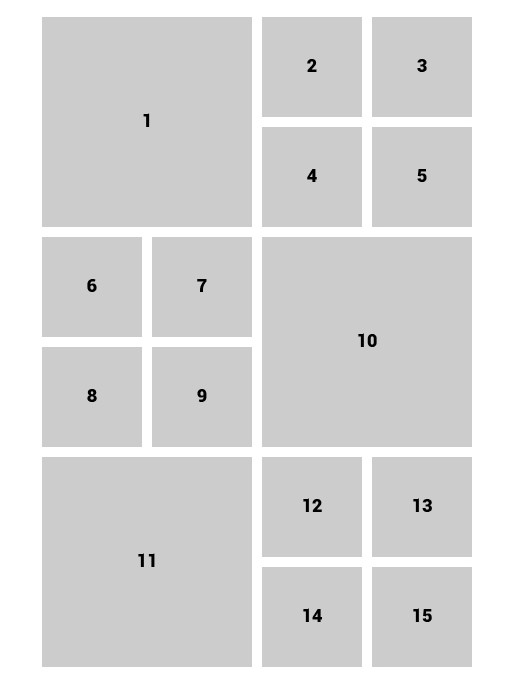
\includegraphics[height=0.4\textheight]{assets/images/theoretical2/css-layout.jpg}
  \caption{Пример сложного позиционирования элементов на странице}
  \label{img:css__layout}
\end{figure}

Также при позиционировании элементов на странице можно применять комбинацию grid и flex моделей. Например, с используя flex можно легче позиционировать элементы в меню, списках, панели навигации и т.д., а grid использовать для основного наполнения страницы, где применение flex будет затруднительно.